\section{Testy statystyczne: EUC2D dla 2-opt i rozszerzonego sąsiada}
  \subsection{Cel:}
    Bazując na wiedzy teoretycznej wiemy, iż 2-opt dla rozkładu miast spełniającego nierówność trójkatą powienien otrzymywać lepsze wyniki niż rozszerzony algorytm najbliższego sąsiada, ze względu na to, iż potrafi on dokonać przestawienia wierzchołków, aby nie dochodziło do potencjalnych przecieć na trasie. Celem tego etapu jest sprawdzenie, czy ta hipoteza jest zgodna z rzeczywistością.
  \subsection{Założenia:}
    Do tego badania użyto automatycznie wygenerowanych grafów typu \textbf{EUC2D}. Rozmiary grafów (oznaczane literą n) należą do zbioru $n \in \{10,15,20,...,100\}$. Dla algorytmu 2-opt element startowy został automatycznie wygenerowany.
  \subsection{Wyniki: }


  \begin{table}[H]
    \begin{tabular}{|c | c | c |} 
     \hline
     n & RozszerzonySąsiad & 2-OPT \\ [0.5ex] 
     \hline\hline
      10 & 271 & 271 \\
      15 & 300 & 300 \\
      20 & 354 & 330 \\
      25 & 408 & 387 \\
      30 & 419 & 414 \\
      35 & 444 & 439 \\
      40 & 458 & 453 \\
      45 & 537 & 513 \\
      50 & 548 & 522 \\
      55 & 573 & 526 \\
      60 & 627 & 563 \\
      65 & 670 & 598 \\ 
      70 & 697 & 630 \\
      75 & 696 & 656 \\
      80 & 752 & 680 \\
      85 & 801 & 712 \\
      90 & 835 & 757 \\
      95 & 949 & 798 \\
      100 & 877 & 821 \\

     \hline
    \end{tabular}
    \caption{Funkcje celu dla wybranych algorytmów.}
    \end{table}

  \subsection{Wykresy: }
  \begin{figure}[H]
      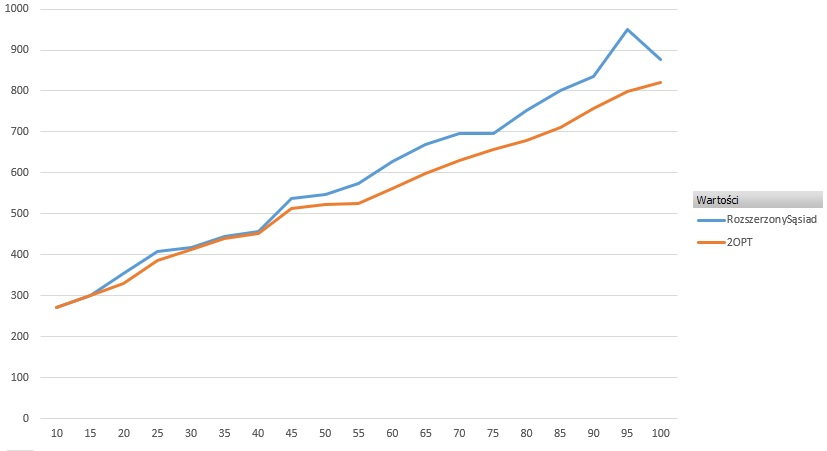
\includegraphics[scale=0.75]{eucOPT}
      \centering
      \caption{Funkcja celu dla 2-opt dla różnych startowych permutacji}
    \end{figure}



  \subsection{Test statystyczny Wilcoxona: }
    \textbf{Hipoteza zerowa: $OPT =< ENN$}, gdzie OPT oznacza algorytm 2-opt, a ENN- rozszerzony algorytm najbliższego sąsiada. \\
    \textbf{Hipoteza alternatywna: $OPT > ENN$ }
    \begin{table}
    \begin{tabular}{|c | c | c | c | c | c |} 
     \hline
     Pair & OPT & ENN & Abs.Diff & Rank & Sign \\ [0.5ex] 
     \hline\hline
      5 & 414 & 419 & 5 & 2 & -1 \\
      6 & 439 & 444 & 5 & 2 & -1 \\
      7 & 453 & 458 & 5 & 2 & -1 \\
      4 & 387 & 408 & 21 & 4 & -1 \\
      3 & 330 & 354 & 24 & 5.5 & -1 \\
      8 & 513 & 537 & 24 & 5.5 & -1 \\
      9 & 522 & 548 & 26 & 7 & -1 \\
      14 & 656 & 696 & 40 & 8 & -1 \\
      10 & 526 & 573 & 47 & 9 & -1 \\
      11 & 563 & 627 & 64 & 11 & -1 \\
      13 & 630 & 697 & 67 & 12 & -1 \\
      12 & 598 & 670 & 72 & 13.5 & -1 \\
      15 & 680& 752 & 72 & 13.5 & -1 \\
      17 & 757 & 835 & 78 & 15 & -1 \\
      16 & 712 & 801 & 89 & 16 & -1 \\
      18 & 798 & 949 & 151 & 17 & -1 \\
     \hline
    \end{tabular}
    \caption{Tabela rang dla testu Wilcoxona}
    \end{table}

    $W_{-} = 153$.\\
    $W_{+} = 0$. \\
  \subsection{Wnioski: }
    Wartość krytyczna $\alpha = 0.05$. Dla tego typu statystyk $T_{crit}=41$ (dana z tabeli dla hipotez "o jednym ogonie"). Hipoteza zerowa jest odrzucona, gdy $ T \leq 41 $. U nas $T=0$, jako minimum z $W_{-} i W_{+}$, więc hipoteza zerowa zostaje odrzucona. Jest wystarczająco powodów na to, aby uważać, iż różnica median jest większa od 0. 